%\documentclass[preprint]{aastex}  % USE THIS TO MAKE BIB, THEN FORMAT USING EMULATEAPJ
\documentclass[twocolumn,numberedappendix]{emulateapj}
\shorttitle{PSA64}
\shortauthors{Parsons, et al.}

\usepackage{amsmath}
\usepackage{graphicx}
\usepackage[figuresright]{rotating}
%\usepackage{rotating}
\usepackage{natbib}
%\usepackage{pdflscape}
%\usepackage{lscape}
\citestyle{aa}

\def\b{\mathbf{b}}
\def\k{\mathbf{k}}
\def\r{\mathbf{r}}
\def\q{\mathbf{q}}
\def\b{\mathbf{b}}
\def\kp{\mathbf{k}^\prime}
\def\kpp{\mathbf{k}^{\prime\prime}}
\def\V{\mathbb{V}}
\def\At{\tilde{A}}
\def\Vt{\tilde{V}}
\def\Tt{\tilde{T}}
\def\tb{\langle T_b\rangle}
\newcommand{\vis}{\mathbf{v}}
\newcommand{\x}{\mathbf{x}}
\newcommand{\xhat}{\hat{\mathbf{x}}}
\newcommand{\A}{\mathbf{A}}
\newcommand{\N}{\mathbf{N}}
\newcommand{\rhat}{\hat{\mathbf{r}}}

\begin{document}
\title{PSA-64 Power Spectrum}

\author{
Zaki S. Ali\altaffilmark{1},
Aaron R. Parsons\altaffilmark{1,2},
Adrian Liu\altaffilmark{1},
James E. Aguirre\altaffilmark{3},
David R. DeBoer\altaffilmark{2},
Daniel C. Jacobs\altaffilmark{8},
David F. Moore\altaffilmark{3},
Jonathan C. Pober\altaffilmark{4},
% XXX if includes paper data, needs full author list
}

\altaffiltext{1}{Astronomy Dept., U. California, Berkeley, CA}
\altaffiltext{2}{Radio Astronomy Lab., U. California, Berkeley, CA}
\altaffiltext{3}{Dept. of Physics and Astronomy, U. Pennsylvania, Philadelphia, PA}
\altaffiltext{4}{Physics Dept.  U. Washington, Seattle, WA}
\altaffiltext{8}{School of Earth and Space Exploration, Arizona State U., Tempe, AZ}

\begin{abstract}
\end{abstract}

% XXX fringe weighting profile
% XXX delay spectrum not violated by freq-dependent fringe rate weights

\section{Introduction}
The Donald C. Backer Precision Array for Probing the Epoch of Reionization
(PAPER) is a dedicated experiment to measure the power spectrum of highly
redshifted 21 cm emission from the Epoch of Reionization.


\section{Observations}
Here, we describe the features of the data set used in this analysis. 
We used the maximally redundant configuration of the PAPER array (see Figure
\ref{fig:antenna_positions} for this analysis, relying on all of the redundant
baselines for the calibration procedure, but only using a subset of the
baselines for the power spectrum analysis. For the power spectrum analysis we
are using the baselines that correspond to the width between two columns (e.g.
49-41) as well as those that correspond to over and up and down one antenna
(e.g. 10-41 and 10-58, respectively). These 154 baselines are used in the power
spectrum analysis because they are instantaneously redundant and therefore they
measure the same Fourier modes on the sky. The sensitivity of the array is mostly
captured by these baselines. 

The observation of the 64 antenna data set spanned a 135 day period that
commenced on 2012 November 8 (JD62456240) and ended  2013 March 23 (JD62456375). 
Each baseline instantaneously measured the 100-200 MHz band which was divided
into 1024 frequency channels of resolution 97.66 kHz and integrated for 10.7
seconds.  

\begin{figure*}\centering
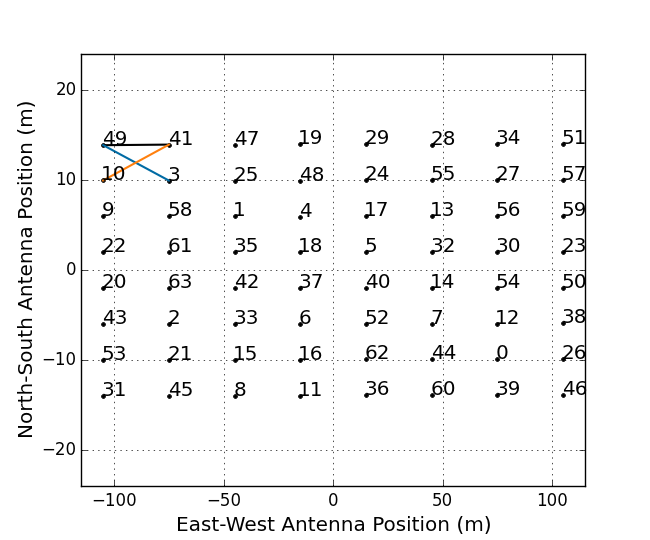
\includegraphics[width=1.85\columnwidth]{plots/antenna_positions.png}
\caption{Antenna positions for the PAPER 64 observation run.}
\label{fig:antenna_positions}
\end{figure*}


\section{Calibrations}
\subsection{General}
The calibration pipeline included a rough calibration based on logarithmic and
linear redundant calibration, as well as self calibration. A rough pass of log
cal was first applied to the data on the basis of redundancy to match up
baselines of the same separation. This included a gain calibration that set the
flux scale to PictorA (Jacobs, 2013).

\subsection{Gain Calibration}
Gain calibration was derived on the basis of redundancy and self calibration.



%\clearpage
\bibliographystyle{apj}
\bibliography{biblio}

\end{document}

